\documentclass[svgnames,tikz]{standalone}
\usetikzlibrary{positioning}

\tikzset{
  focus/.style args={#1 at #2}{
    insert path={
      %{ [white] (#2.north east) rectangle (#2.south west)}
      ($(#2.center)!#1!(#2.north east) $) rectangle ($(#2.center)!#1!(#2.south west) $)
    }
  },
  focusout/.style args={#1 at #2}{
    even odd rule,
    insert path={
      (#2.north east) rectangle (#2.south west)
      ($(#2.center)!#1!(#2.north east) $) rectangle ($(#2.center)!#1!(#2.south west) $)
    }
  },
  txt/.style={font=\Large\tt},
  img/.style={
     inner sep=2pt,
     draw,
     label/.append style={font=\small\tt},
  },
}


\begin{document}
\begin{tikzpicture}
  \tikzset{
    Box/.style={draw, align=center, minimum height=30pt},
    TitleBox/.style={Box, fill=LightGray},
    ImageBox/.style={Box, fill=LightBlue},
    ViewBox/.style={Box, fill=Thistle},
    AlgoBox/.style={Box, fill=LightGreen}
  };


  \node[TitleBox] (A0) []            { Pipeline };
  \node[ImageBox] (A1) [below=of A0] { Input };
  \node[ViewBox]  (A2) [below=of A1] { Select green\\ channel };
  \node[AlgoBox]  (A3) [below=of A2] { Blurring };

  % \draw[-latex] (A0) -- (A1);
  \draw[-latex] (A1) -- (A2);
  \draw[-latex] (A2) -- (A3);


  \node[TitleBox] (A4) [right=of A0] { Memory };
  \node[img]      (A5) [below=of A4] { 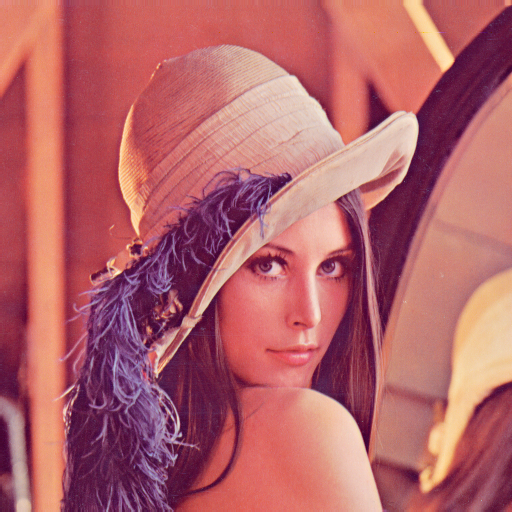
\includegraphics[width=1cm]{../images/lena_color.png} };
  \node[img]      (A6) [below=of A5] { 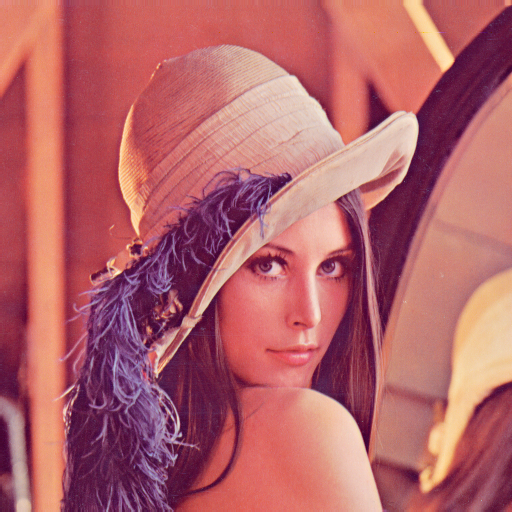
\includegraphics[width=1cm]{../images/lena_color.png} };
  \node[img]      (A7) [below=of A6] { 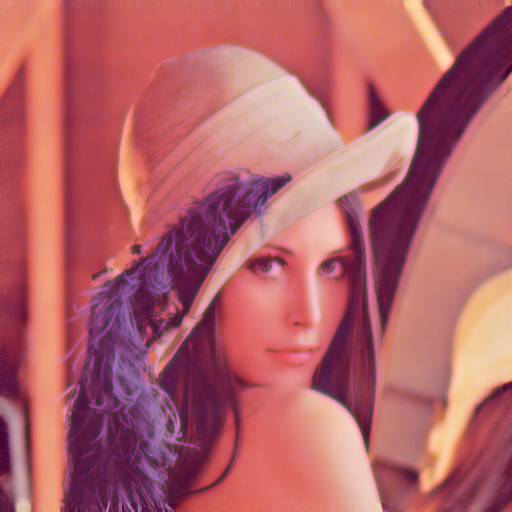
\includegraphics[width=1cm]{../images/lena_color_gblurred.png} };

\end{tikzpicture}
\end{document}
